\let\negmedspace\undefined
\let\negthickspace\undefined
\documentclass[journal,12pt,twocolumn]{IEEEtran}
\usepackage{cite}
\usepackage{amsmath,amssymb,amsfonts,amsthm}
\usepackage{algorithmic}
\usepackage{graphicx}
\usepackage{textcomp}
\usepackage{xcolor}
\usepackage{txfonts}
\usepackage{listings}
\usepackage{enumitem}
\usepackage{mathtools}
\usepackage{gensymb}
\usepackage{comment}
\usepackage[breaklinks=true]{hyperref}
\usepackage{tkz-euclide} 
\usepackage{listings}
\usepackage{gvv}                                        
\def\inputGnumericTable{}                                 
\usepackage[latin1]{inputenc}                                
\usepackage{color}                                            
\usepackage{array}                                            
\usepackage{longtable}                                       
\usepackage{calc}                                             
\usepackage{multirow}                                         
\usepackage{hhline}                                           
\usepackage{ifthen}                                           
\usepackage{lscape}
\usepackage{caption}

\newtheorem{theorem}{Theorem}[section]
\newtheorem{problem}{Problem}
\newtheorem{proposition}{Proposition}[section]
\newtheorem{lemma}{Lemma}[section]
\newtheorem{corollary}[theorem]{Corollary}
\newtheorem{example}{Example}[section]
\newtheorem{definition}[problem]{Definition}
\newcommand{\BEQA}{\begin{eqnarray}}
\newcommand{\EEQA}{\end{eqnarray}}
\newcommand{\define}{\stackrel{\triangle}{=}}
\theoremstyle{remark}
\newtheorem{rem}{Remark}
\begin{document}

\bibliographystyle{IEEEtran}
\vspace{3cm}

\title{10.5.4}
\author{EE23BTECH11029 - Kanishk}
\maketitle
\newpage

\bigskip

\renewcommand{\thefigure}{\theenumi}
\renewcommand{\thetable}{\theenumi}
\textbf{Question}:\\
The houses of a row are numbered consecutively from 1 to 49. Show that there is a value
of x such that the sum of the numbers of the houses preceding the house numbered is equal to the sum of the numbers of the houses following it. Find this value of $x$.\\
Hint:$ S_{x-1}=S_{49}-S_x$

\textbf{Solution}:\\

\begin{table}[ht]
    \centering
    \def\arraystretch{2.5}
    \begin{tabular}{|c|c|c|}
\hline
Parameter & Value & Description \\
\hline
$x\brak{0}$ & $1$ & First term\\
\hline
$d$ & $0$ & Common difference\\
\hline
$x\brak{n}$ & $\sbrak{n+1}u\brak{n}$ & General  term of series \\
\hline
$y\brak{x-2}$ & $\frac{x-1}{2}\brak{x}$ & Sum of x-1 terms \\
\hline
$y\brak{x-1}$ & $\frac{x}{2}\brak{x+1}$ & Sum of x terms. \\
\hline
\end{tabular}

   \caption{Input Parameters}
   \label{tab:10.5.4}
\end{table}

For an AP: 
\begin{align}
X\brak{z}&=\frac{x\brak{0}}{1-z^{-1}}+ \frac{dz^{-1}}{\brak{1-z^{-1}}^{2}}\\
\implies X\brak{z}&=\frac{1}{1-z^{-1}}+ \frac{z^{-1}}{\brak{1-z^{-1}}^{2}}\\
&=\frac{1}{\brak{1-z^{-1}}^{2}},\quad \abs{z} > 1
\end{align}

\begin{align}
    \therefore y\brak{n}=\frac{n+1}{2}\brak{n+2}
\end{align}

\begin{align}
y\brak{x-2}&=y\brak{n-1}-y\brak{x-1}
\end{align}


From \tabref{tab:10.5.4}:

\begin{align}
\brak{\frac{x-1}{2}}x&=\frac{n}{2}\brak{n+1}-\frac{x}{2}\brak{x+1}\\
\brak{x-1}+x\brak{x+1}&=n\brak{n+1}\\
2x^{2}&=n\brak{n+1}\\
x&=\sqrt{\frac{n}{2}\brak{n+1}}
\end{align}

\begin{figure}[h]
    
    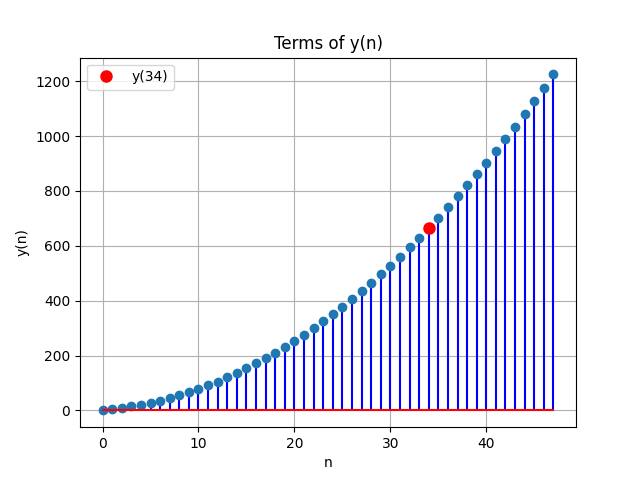
\includegraphics[width=\columnwidth]{figs/fig1.png}
    \caption{Plot y(n) vs n}
\end{figure}

 \end{document}